\documentclass[xcolor=dvipsnames,aspectratio=169,t]{beamer}
  % t means frames are vertically centered to the top
\usepackage{slides-header}
\title{Vector Equations}

\begin{document}
\maketitle

\begin{frame}{Vectors}
  \bbox
  A \alert{vector} is a quantity that has both a length (also called magnitude) and a direction.
  \ebox

  \begin{columns}[T]

    \column{0.33\tw}

    A car is traveling 60 miles per hour directly East.

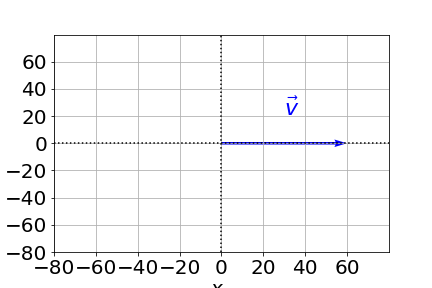
\includegraphics[width=0.9\tw]{images/fig-east.png}

\colorb{    \[ \mathbf{v} = \vec{v} = \begin{bmatrix} 60 \\ 0 \end{bmatrix} \]}


    \column{0.33\tw}

    A car is traveling 40 miles per hour directly South.

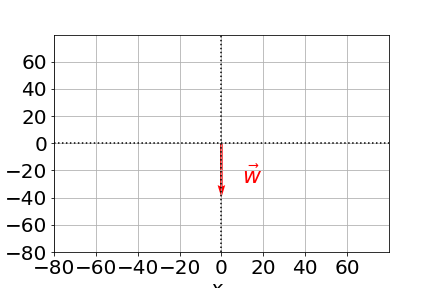
\includegraphics[width=0.95\tw]{images/fig-south.png}

\colorr{    \[ \mathbf{w} = \vec{w} = \begin{bmatrix} 0 \\ -40 \end{bmatrix} \]}
    
    \column{0.33\tw}

    A car is traveling 64 miles per hour directly Northwest.

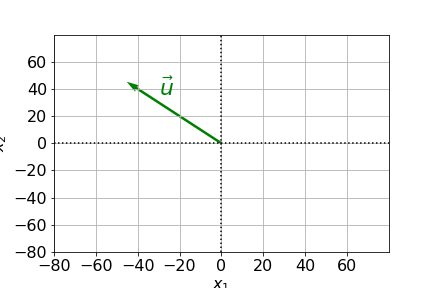
\includegraphics[width=0.95\tw]{images/fig-northwest.png}

\colorg{    \[ \mathbf{u} = \vec{u} = \begin{bmatrix} -\frac{64}{\sqrt{2}}  \\ \frac{64}{\sqrt{2}}  \end{bmatrix} \]}

\end{columns}
    
\end{frame}

\begin{frame}{Vectors in $\mathbb{R}^n$}

  \bbox
  A \alert{vector} (or a \alert{column vector}) is a matrix with only one column.
  \bi
    \ii We denote vectors in bold such as $\mathbf{v}$, and/or
    \ii Using an arrow superscript such as $\vec{v}$.
  \ei
  \ebox

\vfill
  
  \pause
  \bi
  \ii The vector $\dsty \vec{v} = \begin{bmatrix} -12 \\ 8 \end{bmatrix}$ consists of an ordered pair of two real numbers. We say $\vec{v}$ is in $\mathbb{R}^2$ (read as ``r two'' or ``r squared'').
  \ii If the vector $\vec{v}$ consists of $n$ different real numbers, then we have
  \[ \vec{v} = \begin{bmatrix} v_1 \\ v_2 \\ \vdots \\ v_n \end{bmatrix} \in \mathbb{R}^n.\]
  \ei

\end{frame}
  
\begin{frame}{Equality of Vectors}
  
  \bbox
  We say that two vectors $\vec{v} = \begin{bmatrix} v_1 \\ \vdots \\ v_n \end{bmatrix}$ and $\vec{w}= \begin{bmatrix} w_1 \\ \vdots \\ w_n \end{bmatrix}$ are \alert{equal} if:
  \bi
  \ii  They have both the \alert{same direction and the same length}, or equivalently,
  \ii All corresponding entries of the two vectors are equal:
 \alert{  \[ v_i = w_i \ \ \mbox{for all } 1 \leq i \leq n.\] }
  \ei
  \ebox

 \end{frame}


\begin{frame}{Vector Addition}

  {\small
  Given two vectors $\mbf{u} = \begin{bmatrix}u_1\\ \vdots \\ u_n \end{bmatrix}$ and $\mbf{v} = \begin{bmatrix}v_1\\ \vdots \\ v_n \end{bmatrix}$ in $\mathbb{R}^n$, we define their sum as the vector $\mbf{u} + \mbf{v} = \begin{bmatrix} u_1 + v_1 \\ u_2 + v_2 \\ \vdots \\ u_n + v_n \end{bmatrix}$.}

  \pause
  \begin{example}
    Add the vectors.
    \begin{tasks}(2)
    \task $\mathbf{u} = \bbm 2 \\ 2 \ebm$ and $\mbf{v} = \bbm -6 \\ 2 \ebm$. 
    \task $\mathbf{u} = \bbm 1 \\ -3 \\ 8 \\ 0  \ebm$ and $\mbf{v} = \bbm 8 \\ 2 \\ -1 \\ 3 \ebm$.
    \end{tasks}
  \end{example}

  \vfill
     
  \pause
  \bi
    \ii We can only add two vectors if they have the same \alert{dimensions}.
    \ii When we add two vectors, the result is a vector with the same number of dimensions.
  \ei
\end{frame}

\begin{frame}{Scalar Multiplication}

A quantity that has only a magnitude (and does not have a direction) is called a \alert{scalar}. We usually refer to scalars as numbers. For example, $-4$, $\sqrt{5}$, $0$, and $e^2$ are all scalars.

{\small  
  Given a vector $\mbf{v} = \begin{bmatrix} v_1\\ \vdots \\ v_n \end{bmatrix}$ and scalar $c$, we define the \alert{scalar product} of $c$ and $\mbf{v}$ as $c \mbf{v} = \begin{bmatrix} c \cdot v_1 \\ c \cdot v_2 \\ \vdots \\ c \cdot  v_n \end{bmatrix}$. }

  \pause
  \begin{example}
  Compute the scalar product
    \begin{tasks}(2)
    \task $c = -3$ and $\mathbf{v} = \bbm 2 \\ -5 \ebm$. 
    \task $c = 2$ and $\mbf{v} = \bbm 2 \\ 3 \\ 4 \ebm$.
    \end{tasks}
  \end{example}

  \vfill
     
  \pause
  \bi
    \ii We can multiply any scalar and any vector.
    \ii The result is a vector with the same dimension as the original vector.
  \ei
\end{frame}


\begin{frame}{Geometric Descriptions of Vectors in $\mathbb{R}^2$}

{\small  We can think of the vector $\mbf{v} = \bbm v_1 \\ v_2 \ebm \in \mathbb{R}^2$ as a directed line segment (an arrow).}  %with an initial point at the origin $(0,0)$ and terminal point $(v_1, v_2)$.

  \begin{columns}
    
 \column{0.45\tw}
 {\small Consider two vectors $\mbf{u}$ and $\mbf{v} \in \mathbb{R}^2$. The sum $\mbf{u} + \mbf{v}$ is  the result of first moving $\mbf{u}$ and then moving $\mbf{v}$.}

 \onslide<2->{
 \column{0.55\tw}

 {\small Consider the vector $\mbf{u} \in \mathbb{R}^2$ and nonzero scalar $c$. The scalar product $c \mbf{u}$ gives a vector parallel to $\mbf{u}$ whose magnitude has been scaled by a factor of $c$.
 \bi
 \ii If $c > 0$,  then $c \mbf{u}$ has the same direction as $\mbf{u}$.
 \ii If $c < 0$,  then $c \mbf{u}$ has the opposite direction as $\mbf{u}$.
\ii If $|c| < 1$, then $c \mbf{u}$ is a compression of $\mbf{u}$.
\ii If $|c| > 1$, then $c \mbf{u}$ is a stretching of $\mbf{u}$.
\ei }
  }
  \end{columns}

\bbox
{\small  \alert{Parallelogram Rule for Addition:} If $\mbf{u}$ and $\mbf{v}$ are in $\mathbb{R}^2$, then the sum $\mbf{u+v}$ is the diagonal of the parallelogram spanned by $\mbf{u}$ and $\mbf{v}$. }
 \ebox
  
\end{frame}

\begin{frame}{Properties of Vector Arithmetic}

  \bbox
  The \alert{zero vector} is defined as the vector in $\mathbb{R}^n$ with no magnitude, and it is denoted by $\mbf{0}$ or $\vec{0}$. As a result of this definition, it follows that $\dsty \mbf{0} = \bbm 0 \\ 0 \\ \vdots \\ 0 \ebm$.
  \ebox
  \medskip
  
  \pause
  For all $\mbf{u}, \mbf{v}, \mbf{w}$ in $\mathbb{R}^n$ and all scalars $c$ and $d$:

  \begin{columns}[T]
    \column{0.5\tw}
    \begin{enumerate}[(i)]
      \ii $\mbf{u} + \mbf{v} = \mbf{v} + \mbf{u}$
      \ii $(\mbf{u} + \mbf{v}) + \mbf{w} = \mbf{u} + (\mbf{v} + \mbf{w})$
      \ii $\mbf{u} + \mbf{0} = \mbf{0} + \mbf{u} = \mbf{u}$
      \ii $\mbf{u} + (-\mbf{u}) = \mbf{0}$
      \end{enumerate}

    \column{0.5\tw}
    \bb[(i)]
    \setcounter{enumi}{4}
    \ii $c(\mbf{u}+\mbf{v}) = c\mbf{u}+c\mbf{v}$
    \ii $(c+d) \mbf{u} = c\mbf{u} + d \mbf{u}$
    \ii $c(d \mbf{u}) = (cd) \mbf{u}$
    \ii $1 \mbf{u} = \mbf{u}$
    \ee
  \end{columns}

  \end{frame}

\begin{frame}{Giving Directions in Box-Grid City}

  \begin{columns}[T]
    \column{0.5\tw}
  
  \begin{example}

    Find constants $x_1$ and $x_2$ such that
    \[ \bbm -4 \\ -5 \ebm = x_1 \bbm 1 \\ 0 \ebm + x_2 \bbm 0 \\ 1 \ebm .\]
\end{example}

  \column{0.5\tw}

  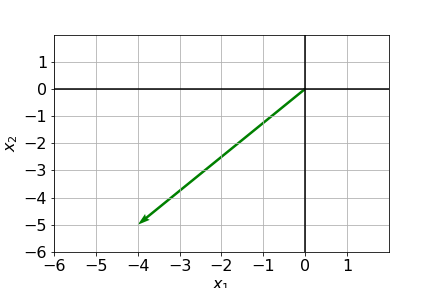
\includegraphics[width=0.95\tw]{images/fig-span1.png}

  \end{columns}

  \vfill
  
  \pause
  \bbox
  The vectors $e_1 = \bbm 1 \\ 0 \ebm$ and $e_2 = \bbm 0 \\ 1 \ebm$ are called \alert{standard column vectors}.
  \ebox

  \end{frame}

\begin{frame}{Giving Directions in Diagonaland}

  \begin{columns}[T]
    \column{0.4\tw}

    {\small
  \begin{example}

    Find constants $x_1$ and $x_2$ such that
    \[ \bbm -4 \\ -5 \ebm = x_1 \bbm 2 \\ 1 \ebm + x_2 \bbm -1 \\ 1 \ebm .\]
\end{example} }

  \column{0.6\tw}

  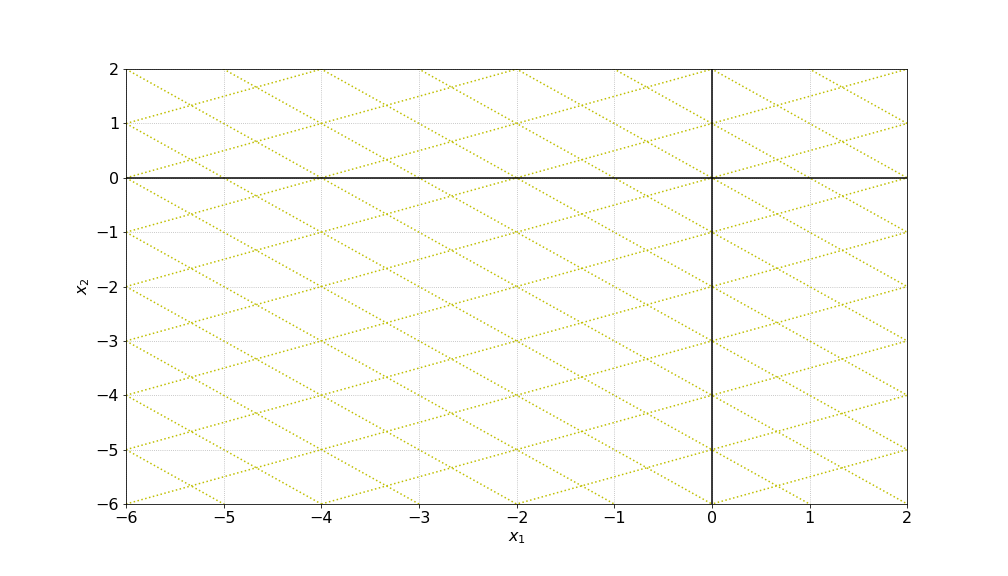
\includegraphics[width=0.95\tw]{images/fig-span2.png}

  \end{columns}

  \vspace{2in}

  \end{frame}

\begin{frame}{Setting up a System of Equations}

  \begin{columns}[T]
    \column{0.5\tw}

    {\small
  \begin{example}

    Find constants $x_1$ and $x_2$ such that
    \[ \bbm -4 \\ -5 \ebm = x_1 \bbm 2 \\ 1 \ebm + x_2 \bbm -1 \\ 1 \ebm .\]
\end{example} }

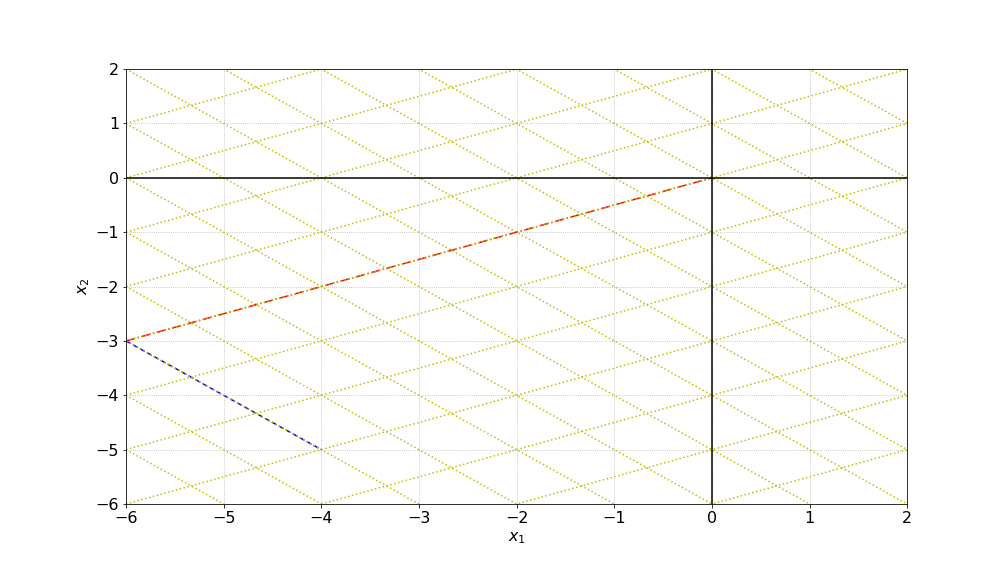
\includegraphics[width=0.95\tw]{images/fig-span3.png}
    
  \column{0.5\tw}
{\small 
  \[  \begin{array}{rcl}
      2x_1 -x_2 &=& -4 \\
      x_1+x_2 &=& - 5 \end{array} \]

  \[ \bbm 2 & - 1 & -4 \\
  1 & 1 & -5
  \ebm \]

  \[ \bbm 1 & 0 & -3 \\
  0 & 1 & -2 \ebm \]

 \[ \mbox{Thus, }  \left\{ \begin{array}{l}
  \alert{x_1 = -3}\\
  \colorb{x_2 = -2}  \end{array} \right. \]

 \vfill

 \alert{Given any vector $\mbf{w}$ in $\mathbb{R}^2$, we can find constants $x_1$ and $x_2$ such that
   \[ \mbf{w} = x_1 \bbm 2 \\ 1 \ebm + x_2 \bbm -1 \\ 1 \ebm . \] } }
 
  \end{columns}

  \vspace{2in}


  \end{frame}

\begin{frame}{Linear Combinations}

  \begin{columns}[T]

    \column{0.5\tw}
    
  {\small  
  \bbox
  Given vectors $\mbf{v}_1, \mbf{v}_2, \ldots , \mbf{v}_p $ in $\mathbb{R}^n$ and scalars $c_1, c_2, \ldots , c_p$, the vector $\mbf{y}$ defined by
  \[ \mbf{y} = c_1 \mbf{v}_1 + c_2 \mbf{v}_2 + \ldots + c_p \mbf{v}_p = \sum_{i=1}^p c_i \mbf{v}_i \]
  is called a \alert{linear combination} of the vectors $\mbf{v}_1, \mbf{v}_2, \ldots , \mbf{v}_p $ with weights $c_1, c_2, \ldots , c_p$.
  \ebox

\alert{Can you think of two different vectors in $\mathbb{R}^2$ such that $\dsty \mbf{w} = \bbm 2 \\ -3 \ebm$ \textbf{cannot} be written as a linear combination of the two vectors?} }
  
  \column{0.5\tw}

  {\small 
  For example: 
%  \[ \bbm -4 \\ -5 \ebm = -3 \bbm 2 \\ 1 \ebm  -2 \bbm -1 \\ 1 \ebm \]
  %we say $\dsty \bbm -4 \\ -5 \ebm$ is linear combination of $\dsty \mbf{v}_1 = \bbm 2 \\ 1 \ebm$ and $\dsty \mbf{v}_2 = \bbm -1 \\ 1 \ebm$ with weights $c_1 = -3$ and $c_2=-2$.

  \[ \bbm 2 \\ -3 \ebm = -\frac{1}{3} \bbm 2 \\ 1 \ebm - \frac{8}{3} \bbm -1 \\ 1 \ebm \] }

  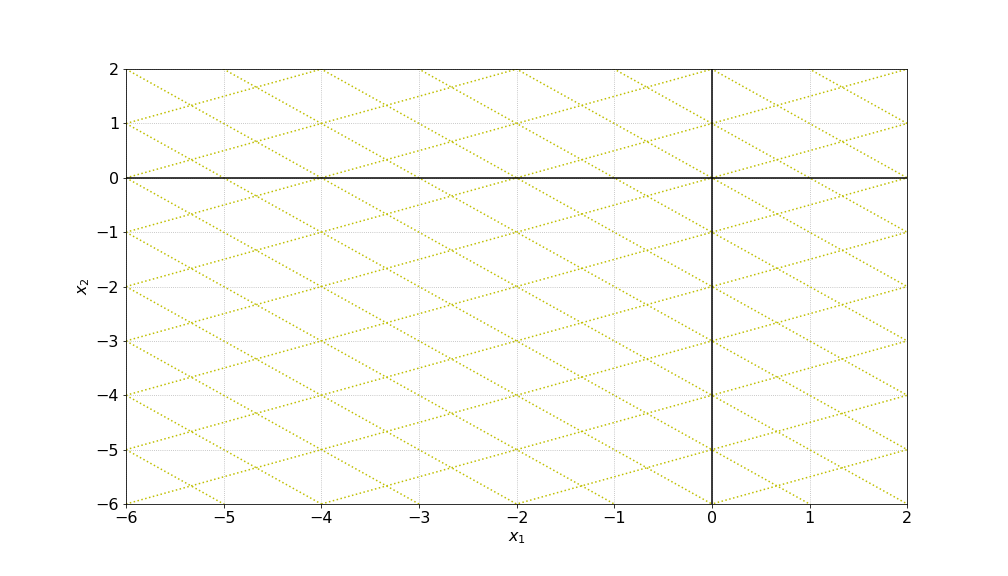
\includegraphics[width=0.9\tw]{images/fig-span2.png}

  
\end{columns}
  
\end{frame}


\begin{frame}{The Span of a Set of Vectors}

  \bbox
  Let $\mbf{v}_1, \mbf{v}_2, \ldots , \mbf{v}_p$ be vectors in $\mathbb{R}^n$. The set of all linear combinations of the vectors $\mbf{v}_1, \mbf{v}_2, \ldots , \mbf{v}_p$ is called the \alert{subset of $\mathbb{R}^n$ spanned by $\mbf{v}_1, \mbf{v}_2, \ldots , \mbf{v}_p$}.

  The set \alert{$\mbox{Span}\lbrace \mbf{v}_1, \mbf{v}_2, \ldots , \mbf{v}_p \rbrace$} is the collection of all vectors in $\mathbb{R}^n$ that can be written in the form
\[  c_1 \mbf{v}_1 + c_2 \mbf{v}_2 + \ldots + c_p \mbf{v}_p = \sum_{i=1}^p c_i \mbf{v}_i. \]
\ebox

  \pause
  To determine whether a vector $\mbf{y}$ is in $\mbox{Span}\lbrace \mbf{v}_1, \mbf{v}_2, \ldots , \mbf{v}_p \rbrace$: 

  \bi
  \ii We try to  solve $c_1 \mbf{v}_1 + c_2 \mbf{v}_2 + \ldots + c_p \mbf{v}_p = \mbf{y}$.
  \ii In other words, we have the augmented matrix 
  \[ \bbm \mbf{v}_1 & \mbf{v}_2 & \ldots & \mbf{v}_p & \mbf{y} \ebm . \] 
  \ei
\end{frame}

\begin{frame}{The Span of a Set of Vectors in $\mathbb{R}^2$}

Describe the span of the set of vectors in $\mathbb{R}^2$.
\bigskip
  
  \begin{tasks}(2)
      \task $\dsty \mbox{Span} \left\{ \bbm 2 \\ 1 \ebm , \bbm -1 \\ 1 \ebm \right\}$  
 \task $\dsty \mbox{Span} \left\{ \bbm 2 \\ 1 \ebm , \bbm -1 \\ 1 \ebm,  \bbm 1 \\ 0 \ebm \right\}$  \vspace{0.75in}
 \task $\dsty \mbox{Span} \left\{ \bbm 2 \\ 1 \ebm , \bbm -4 \\ -2 \ebm \right\}$  
\task $\dsty \mbox{Span} \left\{ \bbm 0 \\ 0 \ebm \right\}$  
\end{tasks}

 \vspace{1.5in}
  
\end{frame}

\begin{frame}{The Span of a Set of Vectors in $\mathbb{R}^3$}

  Describe the span of the set of vectors in $\mathbb{R}^3$.
  \bigskip
  
  \begin{tasks}(2)
 \task $\dsty \mbox{Span} \left\{ \bbm 0 \\ 1 \\ 1 \ebm \right\}$  
 \task $\dsty \mbox{Span} \left\{ \bbm 0 \\ 1 \\ 0 \ebm , \bbm 0 \\ 0 \\ 1 \ebm \right\}$  \vspace{0.7in}
 \task $\dsty \mbox{Span} \left\{  \bbm 1 \\ 0 \\ 0 \ebm , \bbm 0 \\ 1 \\ 0 \ebm , \bbm 0 \\ 0 \\ 1 \ebm \right\}$ 
 \task $\dsty \mbox{Span} \left\{ \bbm 1 \\ 0 \\ -2  \ebm,  \bbm 0 \\ 1 \\ -1  \ebm \right\}$  
\end{tasks}

\vspace{1.5in}

\end{frame}

\begin{frame}{Practice}

  Determine whether the given vector is in $ \mbox{Span} \left\{ \bbm 1 \\ 0 \\ -2  \ebm,  \bbm 0 \\ 1 \\ -1  \ebm \right\}$.
  \bigskip

  \begin{tasks}(2)
    \task $\dsty \bbm 6 \\ -2 \\ -10 \ebm$
    \task $\dsty \bbm 4 \\ 5 \\ -1 \ebm$
  \end{tasks}

\vspace{3in}
  
\end{frame}

\begin{frame}{Conceptual Practice}

Let $\mbf{v}_1, \mbf{v}_2$, $\mbf{v}_3$ and $\mbf{w}$ be vectors in $\mathbb{R}^n$.
Prove that if  $\mbf{w}$ is in $\mbox{Span} \left\{ \mbf{v}_1, \mbf{v}_2, \mbf{v}_3  \right\}$ then $\mbox{Span} \left\{ \mbf{v}_1, \mbf{v}_2 , \mbf{v}_3 , \mbf{w} \right\} = \mbox{Span} \left\{ \mbf{v}_1, \mbf{v}_2 , \mbf{v}_3 \right\}$.

\begin{proof}
\pause
We need to show that the two sets $\mbox{Span} \left\{ \mbf{v}_1, \mbf{v}_2 , \mbf{v}_3 , \mbf{w} \right\}$ and $\mbox{Span} \left\{ \mbf{v}_1, \mbf{v}_2 , \mbf{v}_3 \right\}$ are the same.

($\supseteq$)
Suppose that $\mbf{y}\in \mbox{Span} \left\{ \mbf{v}_1, \mbf{v}_2 , \mbf{v}_3 \right\}$.
Then there exist scalars $c_1, c_2, c_3$ such that $\mbf{y}=c_1 \mbf{v}_1 + c_2 \mbf{v}_2 + c_3 \mbf{v}_3$.
Then $\mbf{y}=c_1 \mbf{v}_1 + c_2 \mbf{v}_2 + c_3 \mbf{v}_3 + 0 \mbf{w}$, and hence $\mbf{y}\in \mbox{Span} \left\{ \mbf{v}_1, \mbf{v}_2 , \mbf{v}_3 , \mbf{w} \right\}$.

\pause
($\subseteq$)
Suppose that $\mbf{y}\in \mbox{Span} \left\{ \mbf{v}_1, \mbf{v}_2 , \mbf{v}_3 , \mbf{w} \right\}$.
Then there exist scalars $c_1, c_2, c_3, d$ such that $\mbf{y}=c_1 \mbf{v}_1 + c_2 \mbf{v}_2 + c_3 \mbf{v}_3 + d \mbf{w}$.
Since $\mbf{w}$ is in $\mbox{Span} \left\{ \mbf{v}_1, \mbf{v}_2, \mbf{v}_3  \right\}$,
there exist scalars $b_1,b_2,b_3$ such that $\mbf{w}=b_1 \mbf{v}_1 + b_2 \mbf{v}_2 + b_3 \mbf{v}_3$.
Substituting for $\mbf{w}$ into the previous equation, we obtain
\vspace*{-1em}\begin{align*}
  \mbf{y}&=c_1 \mbf{v}_1 + c_2 \mbf{v}_2 + c_3 \mbf{v}_3 + d \mbf{w} \\
         &=c_1 \mbf{v}_1 + c_2 \mbf{v}_2 + c_3 \mbf{v}_3 + d \left( b_1 \mbf{v}_1 + b_2 \mbf{v}_2 + b_3 \mbf{v}_3\right) \\
         &= (c_1+db_1) \mbf{v}_1 + (c_2+db_2) \mbf{v}_2 + (c_3+db_3) \mbf{v}_3 .
\end{align*}

\vspace*{-1em}
Since $c_1+db_1$, $c_2+db_2$, and $c_3+db_3$ are scalars, $\mbf{w}$ is a linear combination of $\mbf{v}_1, \mbf{v}_2 , \mbf{v}_3$, and hence $\mbf{y}\in \mbox{Span} \left\{ \mbf{v}_1, \mbf{v}_2 , \mbf{v}_3 \right\}$.
Thus, $\mbox{Span} \left\{ \mbf{v}_1, \mbf{v}_2 , \mbf{v}_3 , \mbf{w} \right\} = \mbox{Span} \left\{ \mbf{v}_1, \mbf{v}_2 , \mbf{v}_3 \right\}$.
\end{proof}

\vspace{3in}

\end{frame}

\begin{frame}{Parametric Vector Form for Solutions of a Linear System}

  Find the solution set to the linear system
  \[
    \begin{array}{ccccccc}
      x_1 & +2x_2 &     &     & -4x_5 &=& 0\\
          &       & x_3 &     & +7x_5 &=& 1 \\   
          &       &     & x_4 & +5x_5 &=& 2
    \end{array}
  \]

  {\small
  \begin{columns}
  \pause
  \column{.3\textwidth}
  \[
    \left\{ \begin{array}{l}
    x_1 = -2x_2 +4x_5\\
    x_2 \text{ is \alert{free}}\\
    x_3 = 1-7x_5 \\
    x_4 = 2-5x_5 \\
    x_5 \text{ is \alert{free}}\\
    \end{array} \right.
  \]
  
  \pause
  \column{.7\textwidth}
  \vspace*{-.5em}%
  \begin{align*}
    \begin{bmatrix} x_1 \\ x_2 \\ x_3 \\ x_4 \\ x_5 \end{bmatrix} 
    = \begin{bmatrix} -2x_2 +4x_5\\ \alert{x_2} \\ 1-7x_5 \\ 2-5x_5 \\ \alert{x_5} \end{bmatrix}
    &= \begin{bmatrix} 0 \\ 0 \\ 1 \\ 2 \\ 0 \end{bmatrix}
    + x_2 \begin{bmatrix} -2 \\ \alert{1} \\ 0 \\ 0 \\ 0 \end{bmatrix}
    + x_5 \begin{bmatrix} 4 \\ 0 \\ -7 \\ -5 \\ \alert{1} \end{bmatrix}\\
    &= \begin{bmatrix} 0 \\ 0 \\ 1 \\ 2 \\ 0 \end{bmatrix}
    + \colorb{s} \begin{bmatrix} -2 \\ \alert{1} \\ 0 \\ 0 \\ 0 \end{bmatrix}
    + \colorb{t} \begin{bmatrix} 4 \\ 0 \\ -7 \\ -5 \\ \alert{1} \end{bmatrix}.
  \end{align*}
  \end{columns}
  }
  \bigskip
  
  \hspace*{10em} The weights $\colorb{s,t}$ are any scalars. This is called \colorb{parametric vector form}.
\end{frame}

\end{document}
